%%% Dateikodierung: UTF-8

%%% Magic Comments zum Setzen der korrekten Parameter in kompatiblen IDEs
% !TeX encoding = utf8
% !TeX program = pdflatex 
% !TeX spellcheck = de_DE
% !BIB program = biber

\RequirePackage[utf8]{inputenc} % bei Verw. von lualatex oder xelatex entfernen!
\RequirePackage{hgbpdfa}				% Remove if NO PDF/A output is desired

\documentclass[type=master,theme=default,language=german,titlelanguage=german,smartquotes]{hgbthesis}
% Zulässige Optionen in [..]: 
%    Typ der Arbeit (type=): 'master' (default), 'bachelor', 'diploma', 'phd', 'internship'
%    Theme der Titelseite (theme=): 'default' (default), 'fhooe24'
%    Als Exposé verwenden: 'proposal' oder 'proposal=true' 
%    Hauptsprache im Dokument (language=): 'german' (default), 'english'
%    Sprache der Titelseite (titlelanguage=): 'german', 'english' (default is main language)
%    Umwandlung in typografische Anführungszeichen: 'smartquotes'
%    APA Zitierstil: 'apa'
%    Layout: 'oneside' (einseitig, default), 'twoside' (zweiseitig)
%%%-----------------------------------------------------------------------------

\graphicspath{{images/}}  % Verzeichnis mit Bildern und Grafiken
\bibliography{hgbreferences} % Biblatex-Literaturdatei (hgbreferences.bib)
\usepackage{pifont}
\newcommand{\cmark}{\ding{51}} % ✓
\newcommand{\xmark}{\ding{55}} % ✗

%%%-----------------------------------------------------------------------------
\begin{document}
%%%-----------------------------------------------------------------------------

%%%-----------------------------------------------------------------------------
% Angaben für die Titelei (Titelseite, Erklärung etc.)
%%%-----------------------------------------------------------------------------

\title{Vorprojektbericht}
\subtitle{Aufbau einer CyberRange als Forschungsumgebung\\
zur Untersuchung von Cyber-Resilienz}
\author{Peter Hartl}

\programtype{Fachhochschul-Masterstudiengang} % oder Fachhochschul-Bachelorstudiengang
\programname{Secure Information Systems}
\institution{Fachhochschule Oberösterreich}

\placeofstudy{Hagenberg}
\dateofsubmission{2026}{01}{30} % {JJJJ}{MM}{TT}

% Liste der Betreuungspersonen, bis zu 4 sind möglich, Titel in [] ist optional
\advisor{FH-Prof.\ DI Robert Kolmhofer}
%\advisor[Zweitbetreuerin]{FH-Prof.\textsuperscript{in} Susanna A.~D. Visor, PhD}

\license{cc}      % Unter Creative Commons Lizenz veröffentlichen (empfohlen)
%\license{strict} % Restriktieve Lizenz, "Alle Rechte vorbehalten"

%%%-----------------------------------------------------------------------------
\frontmatter                                       % Titelei (röm. Seitenzahlen)
%%%-----------------------------------------------------------------------------

\maketitle
\tableofcontents



%%%-----------------------------------------------------------------------------
\mainmatter                             % Hauptteil (ab hier arab. Seitenzahlen)
%%%-----------------------------------------------------------------------------

\chapter{Einleitung}
\label{chap:einleitung}

\section{Motivation und Problemstellung}
\label{sec:motivation}

Mit europäischen Regelwerken wie der NIS-2-Richtlinie~\cite{NIS2Directive},
dem Cyber Resilience Act (CRA)~\cite{CyberResilienceAct} und der Digital
Operational Resilience Regulation (DORA)~\cite{DORARegulation} steigen die
Anforderungen an Organisationen, ihre IT-Systeme nicht nur präventiv abzusichern, sondern deren Widerstandsfähigkeit gegenüber Sicherheitsvorfällen ganzheitlich zu betrachten. Neben klassischen Schutzmaßnahmen rücken dabei insbesondere die Fähigkeiten zur Erkennung, Reaktion und Wiederherstellung nach Sicherheitsvorfällen sowie die Nachweisbarkeit dieser Prozesse in den Vordergrund. Resilienz wird damit zu einer Eigenschaft, die nicht nur konzipiert, sondern auch überprüft werden muss.

Für Forschung und Entwicklung ergibt sich daraus die Frage, wie sich solche Fähigkeiten
unter realistischen, zugleich aber kontrollierten Bedingungen untersuchen und bewerten
lassen. Produktive Systeme sind dafür nur eingeschränkt geeignet, da Sicherheitsvorfälle
dort erhebliche Risiken verursachen können. Gleichzeitig fehlt es an
standardisierten Testumgebungen, die reproduzierbare Experimente im Bereich der
Cyber-Resilienz erlauben \cite{Chouliaras2021}.

Cyber Ranges adressieren dieses Spannungsfeld, indem sie virtuelle, isolierte
IT-Landschaften bereitstellen, in denen Angriffs- und Verteidigungsszenarien realitätsnah
nachgebildet werden können. Während viele existierende Cyber-Range-Plattformen jedoch
primär für Schulungs- und Trainingszwecke entwickelt wurden, ist ihr systematischer
Einsatz als Forschungsumgebung -- insbesondere zur reproduzierbaren Evaluation von
Sicherheitswerkzeugen -- bislang nur teilweise etabliert \cite{IntroductionCyberRanges2022}.

Genau hier setzt die vorliegende Arbeit an. Um Sicherheits- und Analysewerkzeuge
objektiv miteinander vergleichen oder resilienzbezogene Eigenschaften eines Systems
beurteilen zu können, müssen identische Szenarien unter gleichen Randbedingungen
wiederholt ausführbar sein. Fehlt diese Reproduzierbarkeit, lassen sich beobachtete
Unterschiede nicht zweifelsfrei auf das untersuchte Werkzeug zurückführen. Die
Problemstellung besteht somit darin, eine geeignete Cyber-Range-Plattform so aufzubauen
und zu betreiben, dass sie als reproduzierbare Forschungsumgebung für
Cyber-Resilienz-Untersuchungen dienen kann, und dies anhand konkreter, wiederholbarer
Use Cases nachzuweisen.

\section{Zielsetzung}
\label{sec:zielsetzung}

Ziel dieser Arbeit ist es, eine geeignete Cyber-Range-Plattform auszuwählen, aufzubauen
und als reproduzierbare Forschungsumgebung für Fragestellungen der Cyber-Resilienz
nutzbar zu machen. Im Mittelpunkt stehen reproduzierbare Anwendungsszenarien (Use Cases),
an denen sich Sicherheits- und Analysewerkzeuge unter identischen Bedingungen einbinden
und vergleichen lassen sowie die Funktionsfähigkeit der Forschungsumgebung selbst belegen.
Der erste und im Detail ausgearbeitete Use Case ist ein Vergleich von Schwachstellen-Scannern
unterschiedlicher Charakteristik (klassisch, modern und kommerziell) gegen ein definiert
verwundbares Zielsystem.

Konkret verfolgt die Arbeit folgende Teilziele:
\begin{itemize}
  \item Es werden objektive Kriterien zur Bewertung von Cyber-Range-Plattformen aus
        Forschungsperspektive definiert.
  \item Auf dieser Basis wird die am besten geeignete Plattform ausgewählt und als
        Forschungsumgebung implementiert.
  \item Es werden reproduzierbare Cyber-Resilienz-Use-Cases konzipiert und technisch
        umgesetzt, in die externe Sicherheits- bzw.\ Analysewerkzeuge eingebunden werden.
  \item Es wird eine Evaluationsmethodik entwickelt, mit der sich Funktionsfähigkeit und
        Reproduzierbarkeit der Umgebung und der Use Cases überprüfen lassen.
\end{itemize}

Das angestrebte Ergebnis ist eine funktionsfähige, modular erweiterbare Forschungsumgebung,
die wiederholbare Experimente im Bereich der Cyber-Resilienz ermöglicht, gemeinsam mit einer
belastbaren Methodik zu deren Bewertung.

\section{Forschungsfragen}
\label{sec:forschungsfragen}

Aus der Problem- und Zielsetzung leitet sich die folgende übergeordnete Forschungsfrage ab:

\begin{quote}
Wie kann eine geeignete Cyber-Range-Plattform ausgewählt, aufgebaut und eingesetzt werden,
um eine funktionsfähige Forschungsumgebung für Cyber-Resilienz mit reproduzierbaren Use
Cases bereitzustellen?
\end{quote}

Zur Beantwortung der Forschungsfrage werden die folgenden Untersuchungsfragen betrachtet:

\begin{enumerate}
  \item Nach welchen objektiven Kriterien lassen sich Cyber-Range-Plattformen für Forschung
        und Tool-Integration bewerten?
  \item Welche Plattform erfüllt diese Anforderungen am besten und eignet sich für den Aufbau
        einer forschungsorientierten Umgebung?
  \item Wie können realistische und reproduzierbare Cyber-Resilienz-Use-Cases auf der
        ausgewählten Plattform modelliert und umgesetzt werden?
  \item Welche technischen Schnittstellen sind notwendig, um Sicherheits- oder
        Monitoring-Tools in die Cyber Range einzubinden?
  \item Wie lässt sich die Funktionsfähigkeit und Reproduzierbarkeit der entwickelten Use
        Cases evaluieren?
\end{enumerate}

\section{Methodik}
\label{sec:methodik}

Die Arbeit folgt einem \emph{Design-Science-Research}-Ansatz (DSR), der die Konstruktion
und Evaluation eines praktischen Artefakts -- hier der Forschungsumgebung samt Use Cases --
in den Mittelpunkt stellt und mit einer systematischen Literaturrecherche kombiniert
\cite{Hevner2004DesignScience}. Das Vorgehen orientiert sich an den etablierten Phasen
gestaltungsorientierter Forschung \cite{Peffers2007DSRM} und gliedert sich in:

\begin{enumerate}
  \item \textbf{Analyse:} Untersuchung existierender Cyber-Range-Plattformen sowie
        wissenschaftlicher Ansätze zu Szenarienmodellierung, Reproduzierbarkeit und
        Tool-Integration.
  \item \textbf{Plattformvergleich:} strukturierter Vergleich mehrerer Plattformen anhand
        definierter Kriterien und Auswahl der geeignetsten Lösung.
  \item \textbf{Konzeption:} Entwurf reproduzierbarer Cyber-Resilienz-Use-Cases inklusive
        Evaluationskriterien.
  \item \textbf{Implementierung:} technische Umsetzung der Use Cases auf der ausgewählten
        Plattform inklusive der notwendigen Integrationsschnittstellen.
  \item \textbf{Evaluation:} Überprüfung von Funktionsfähigkeit, Reproduzierbarkeit und
        Erweiterbarkeit der entwickelten Umgebung und Use Cases.
  \item \textbf{Reflexion:} Ableitung von Empfehlungen für den wissenschaftlichen Einsatz von
        Cyber Ranges.
\end{enumerate}

\section{Aufbau der Arbeit}
\label{sec:aufbau}

Kapitel~\ref{chap:einleitung} umreißt Motivation, Zielsetzung, Forschungsfragen und Methodik.
Kapitel~\ref{chap:grundlagen} erarbeitet die fachlichen Grundlagen zu Cyber Ranges, Cyber-Resilienz
und Schwachstellen-Scannern. Kapitel~\ref{chap:stand-der-technik} ordnet den Stand der Technik ein,
betrachtet bestehende Cyber-Range-Plattformen und leitet die Forschungslücke ab.
Kapitel~\ref{chap:poc} erprobt die beiden zentralen quelloffenen Kandidaten praktisch in einem Proof
of Concept. Aufbauend darauf entwickelt Kapitel~\ref{chap:auswahl} einen Kriterienkatalog, vergleicht
die Plattformen und begründet die Auswahl. Kapitel~\ref{chap:uc1} setzt den ersten Use Case auf der
gewählten Plattform um und führt von der Konzeption über die Evaluationsmethodik und die
Implementierung bis zu den Ergebnissen und deren Diskussion. Anhang~\ref{chap:quelltext-uc1} enthält
den vollständigen Quelltext der Use-Case-Umgebung.

\chapter{Grundlagen}
\label{chap:grundlagen}

Dieses Kapitel erarbeitet die fachlichen Grundlagen der Arbeit. Abschnitt~\ref{sec:cyber-ranges}
führt in Cyber Ranges ein, ordnet den Begriff ein und grenzt ihn von verwandten Konzepten ab.
Abschnitt~\ref{sec:cyber-resilienz} behandelt Cyber-Resilienz als konzeptionellen Rahmen, und
Abschnitt~\ref{sec:vuln-scanner} legt die Grundlagen zu Schwachstellen-Scannern, die im ersten
Use Case verglichen werden.

\section{Cyber Ranges}
\label{sec:cyber-ranges}

\subsection{Begriff und Abgrenzung}
\label{subsec:cr-begriff}

Cyber Ranges werden als komplexe, virtuelle Umgebungen beschrieben, die reale
Cybersecurity-Situationen -- etwa Angriffe oder Cyberwarfare -- nachbilden und in einem
kontrollierten Rahmen sowohl praxisnahes Training als auch Forschung und die Untersuchung
unterschiedlicher Szenarien ermöglichen \cite[2--3]{IntroductionCyberRanges2022}. Als kennzeichnend
gilt dabei die Kombination aus realitätsnaher Simulation, einer virtuellen Umgebung, in der
mehrere Teams agieren können, sowie einer leistungsbasierten Bewertung der durchgeführten
Übungen \cite[2--3]{IntroductionCyberRanges2022}. In der wissenschaftlichen Literatur werden Cyber
Ranges übereinstimmend als virtuelle, isolierte IT-Landschaften charakterisiert, in denen sich
sicherheitsrelevante Ereignisse analysieren lassen, ohne produktive Systeme zu gefährden
\cite{Chouliaras2021}.

Von klassischen \emph{Testbeds} unterscheiden sich Cyber Ranges weniger durch die zugrunde
liegende technische Infrastruktur als vielmehr durch ihren szenarienorientierten Charakter.
Während Testbeds primär auf die Untersuchung einzelner Technologien oder Netzwerkkonfigurationen
ausgerichtet sind, kombinieren Cyber Ranges Infrastruktur, Benutzerinteraktion und zeitliche
Abläufe innerhalb eines integrierten Szenariokonzepts und eignen sich dadurch für die
Untersuchung komplexer, mehrstufiger Sicherheitsereignisse \cite[2]{Chouliaras2021}. Ähnlich
adressieren \emph{Digital Twins} und Testbeds auf Systemebene typischerweise die Abbildung und
Validierung eines konkreten Systems, während Cyber Ranges primär der reproduzierbaren
Bereitstellung variabler Übungs- und Experimentierumgebungen für Angriffs-, Verteidigungs- und
Evaluationsszenarien dienen.

Ursprünglich wurden Cyber Ranges vor allem für Ausbildungs- und Trainingszwecke entwickelt. In
der Literatur wird jedoch zunehmend ihre Nutzung als Forschungsumgebung hervorgehoben,
insbesondere dann, wenn reproduzierbare Szenarien und strukturierte Bewertungsmechanismen
vorgesehen sind: Durch die kontrollierte, wiederholbare Durchführung identischer Szenarien lassen
sich unterschiedliche Werkzeuge, Strategien oder Vorgehensweisen unter vergleichbaren Bedingungen
untersuchen \cite[2]{Chouliaras2021,Yamin2020CyberRanges}. Ein wesentliches Merkmal moderner
Cyber Ranges ist damit die Verbindung von Lern-, Trainings- und Validierungsaspekten innerhalb
einer gemeinsamen Umgebung \cite{IntroductionCyberRanges2022}.

Für die vorliegende Arbeit ist insbesondere diese forschungsorientierte Perspektive relevant.
Während Trainings- und Testaspekte als notwendige Bestandteile moderner Cyber Ranges betrachtet
werden, liegt der Schwerpunkt hier auf der Nutzung einer Cyber Range als \emph{reproduzierbare
Forschungsumgebung}. Diese Einordnung bildet die begriffliche Grundlage für die weiteren
Abschnitte und für die spätere Ableitung von Anforderungen an die Plattformauswahl.

\subsection{Architektur und Komponenten}
\label{subsec:cr-architektur}

Die konkrete Architektur einer Cyber Range hängt von ihrem Einsatzzweck ab: Eine Plattform
kann sämtliche Funktionen abdecken oder gezielt auf eine Spezialisierung -- etwa Forschung,
Security-Testing ausgerichtet sein \cite[13]{IntroductionCyberRanges2022}.
Übergreifend lässt sich jedoch ein verbreitetes Architekturmodell beschreiben, das aus fünf
funktionalen Modulen besteht \cite[13]{IntroductionCyberRanges2022}:

\begin{itemize}
  \item \textbf{Portal:} stellt die Benutzeroberfläche und die Zugangsschicht bereit; der
        Zugriff auf virtuelle bzw.\ cloud-basierte Cyber Ranges erfolgt typischerweise über
        einen Webbrowser und einen Webserver (z.\,B.\ Nginx oder Apache).
  \item \textbf{Laufzeitumgebung:} führt die Szenarien aus und unterstützt simulationsbasierte Umgebungen sowie die Erzeugung von Netzwerkverkehr zur realitätsnahen
        Nachbildung.
  \item \textbf{Management:} betrifft die Ressourcenzuteilung sowie Team- und Aufgabenverwaltung
        während der Durchführung einer CSE (Cyber Security Exercise).
  \item \textbf{Datenbank:} speichert Übungsmodule, Statistiken und Logs. Eingesetzt werden dabei 
        relationale (MySQL) oder NoSQL-Datenbanken.
  \item \textbf{Monitoring:} erfasst und überwacht den Ablauf der Übungen sowie Mess- und
        Auswertungsdaten für Forschung und Produkttests.
\end{itemize}

Die Laufzeitumgebung stützt sich dabei auf unterschiedliche Werkzeugklassen: Virtualisierungswerkzeuge (z.\,B.\ VMware, VirtualBox, KVM oder QEMU sowie Cloud-Frameworks wie
OpenNebula) bilden Systeme als virtuelle Maschinen ab, Simulationswerkzeuge modellieren das
Verhalten ganzer Netze, und Traffic-Generatoren erzeugen realistischen Datenverkehr
\cite[14--21]{IntroductionCyberRanges2022}. In der Forschungsliteratur wird die Architektur entsprechend
als eine der zentralen Dimensionen zur Charakterisierung von Cyber Ranges geführt -- neben
Szenarien, Funktionen und Werkzeugen \cite{Yamin2020CyberRanges}.

Die in dieser Arbeit eingesetzte Plattform setzt dieses Modell konkret um: Ein Web-Portal bildet
die Zugangsschicht, die Bereitstellung der Szenarien (Sandboxes) erfolgt automatisiert auf einer
virtualisierten Cloud-Infrastruktur, und die Lebenszyklusverwaltung übernehmen dedizierte
Management-Dienste. Diese Umsetzung wird in Kapitel~\ref{chap:stand-der-technik} sowie bei der
Implementierung der Forschungsumgebung gezeigt.

\subsection{Typen von Cyber Ranges}
\label{subsec:cr-typen}

Nach Art der technischen Realisierung lassen sich Cyber Ranges in drei Typen einteilen --
physisch, virtuell und hybrid (Abbildung~\ref{fig:cr-typen})
\cite[47--63]{IntroductionCyberRanges2022}.

\begin{figure}[H]
  \centering
  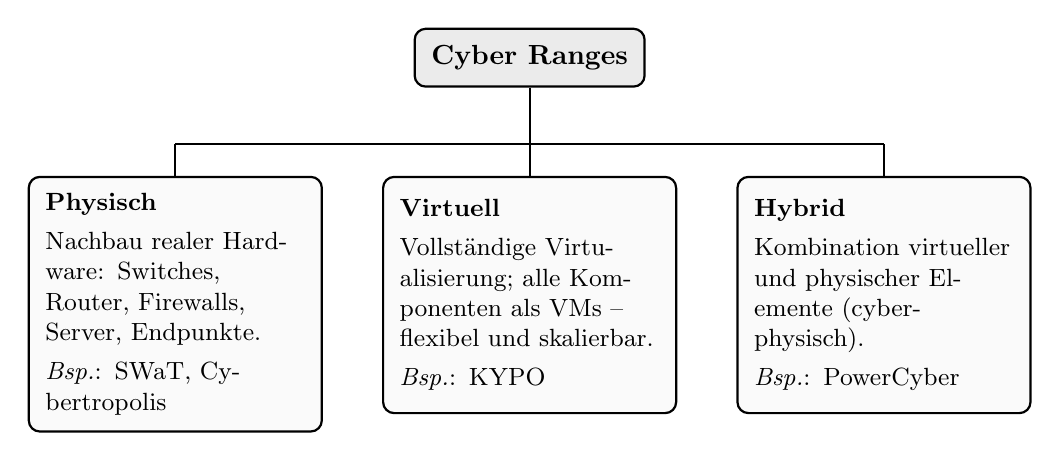
\begin{tikzpicture}[
      font=\small,
      box/.style={
        draw, rounded corners, thick, fill=black!2,
        text width=3.3cm, align=left, inner sep=6pt,
        minimum height=3cm, anchor=north
      },
      root/.style={
        draw, rounded corners, thick, fill=black!8,
        inner sep=6pt, font=\bfseries
      }
    ]
    \node[root] (root) at (0,0) {Cyber Ranges};

    \node[box] (phys) at (-4.5,-1.5) {\textbf{Physisch}\\[3pt]
      Nachbau realer Hardware: Switches, Router, Firewalls, Server,
      Endpunkte.\\[3pt]
      \emph{Bsp.}: SWaT, Cybertropolis};
    \node[box] (virt) at (0,-1.5) {\textbf{Virtuell}\\[3pt]
      Vollständige Virtualisierung; alle Komponenten als VMs -- flexibel
      und skalierbar.\\[3pt]
      \emph{Bsp.}: KYPO};
    \node[box] (hybr) at (4.5,-1.5) {\textbf{Hybrid}\\[3pt]
      Kombination virtueller und physischer Elemente (cyber-physisch).\\[3pt]
      \emph{Bsp.}: PowerCyber};

    \draw[thick] (root.south) -- (0,-1.1);
    \draw[thick] (-4.5,-1.1) -- (4.5,-1.1);
    \draw[thick] (-4.5,-1.1) -- (phys.north);
    \draw[thick] (0,-1.1) -- (virt.north);
    \draw[thick] (4.5,-1.1) -- (hybr.north);
  \end{tikzpicture}
  \caption{Typen von Cyber Ranges (eigene Darstellung in Anlehnung an \cite{IntroductionCyberRanges2022})}
  \label{fig:cr-typen}
\end{figure}

Eine physische Cyber Range bildet die reale Infrastruktur vollständig nach. Komponenten
wie Firewalls, Server und Router werden als echte Hardware dupliziert. Das wirkt sehr realistisch, ist jedoch mit erheblichen Nachteilen verbunden -- hohe Anschaffungs- und
Betriebskosten, großer Strom- und Kühlbedarf sowie aufwändige Auf- und Rückbauprozesse
\cite[54]{IntroductionCyberRanges2022}. Typische Beispiele sind SCADA-Testbeds wie SWaT und WADI
oder die frühe USMA~IWAR.

Eine virtuelle Cyber Range besteht vollständig aus virtualisierten Komponenten, die als
virtuelle Maschinen abgebildet werden. Gegenüber physischen Umgebungen sinken Kosten und Aufwand
deutlich: Umgebungen lassen sich bei Bedarf schnell bereitstellen, nach einer Übung zurücksetzen,
flexibel skalieren und auf handelsüblicher Hardware betreiben \cite[60]{IntroductionCyberRanges2022}.
Als Einschränkung gilt, dass sich nicht jedes Szenario realitätsgetreu nachbilden lässt -- die
exakte Modellierung physischer Komponenten ist im virtuellen Umfeld schwieriger. 

Eine hybride Cyber Range kombiniert virtuelle und physische Elemente (cyber-physische
Range) und vereint so die Skalierbarkeit virtueller Umgebungen mit dem Realismus physischer
Komponenten. Der Anteil beider richtet sich nach den Anforderungen des Szenarios
\cite[47]{IntroductionCyberRanges2022}. Beispiele sind EVA, DIATEAM und CRATE.

Unabhängig vom Typ wird zwischen Betriebsmodellen unterschieden: Bei einer On-Premise-Cyber
Range betreibt die Organisation die Plattform selbst, was maximale Kontrolle ermöglicht, aber
kostenintensiver ist. Cyber Range as a Service(CRaaS) wird hingegen cloudbasiert von einem
Anbieter bereitgestellt und ist schnell und wirtschaftlich verfügbar, geht jedoch mit geringerer
Kontrolle über die Infrastruktur einher \cite[63]{IntroductionCyberRanges2022}. Die vorliegende
Arbeit setzt auf eine virtuelle, selbst betriebene (On-Premise) Cyber Range, da die
Reproduzierbarkeit, Kostenkontrolle und Skalierbarkeit für eine Forschungsumgebung am wichtigsten sind. 

\subsection{Einsatzzwecke: Testing, Training und Forschung}
\label{subsec:cr-einsatzzwecke}

Cyber Ranges werden für drei übergeordnete Einsatzzwecke genutzt -- Testing, Training und
Forschung. Diese unterscheiden sich aber weniger durch die zugrunde liegende Technik als durch Zielsetzung,
Szenariogestaltung und Art der Ergebnisbewertung \cite[67]{IntroductionCyberRanges2022}\cite{Chouliaras2021}.

Im Testing dienen Cyber Ranges der Überprüfung von Systemen, Softwarekomponenten und
Sicherheitsmechanismen. Typische Verfahren sind Penetration-, Software- und Security-Testing \cite[67--72]{IntroductionCyberRanges2022}. 

Im Training steht der Aufbau von Kompetenz im Umgang mit Sicherheitsvorfällen im
Vordergrund -- wie etwa Awareness-Schulungen und Incident-Response-Übungen, in denen Teams unter
realitätsnahen Bedingungen Erkennung, Analyse und Reaktion üben \cite[72]{IntroductionCyberRanges2022}.

Im Forschungskontext werden Cyber Ranges als experimentelle Umgebungen zum systematischen
Erkenntnisgewinn genutzt, um Werkzeuge zu vergleichen oder das Verhalten von Systemen unter
definierten Bedingungen zu analysieren. Zentrale Anforderungen sind dabei Nachvollziehbarkeit und
Reproduzierbarkeit der Szenarien, sodass Ergebnisse nicht nur situationsbezogen interpretiert,
sondern verallgemeinert werden können \cite[76--78]{IntroductionCyberRanges2022}\cite{Chouliaras2021,Yamin2020CyberRanges}.

\section{Cyber-Resilienz}
\label{sec:cyber-resilienz}

\subsection{Begriff und Einordnung}
\label{subsec:resilienz-begriff}

Klassische Sicherheitsansätze zielen vor allem auf Vermeidung und Schutz ab. Cyber-Resilienz geht
einen Schritt weiter. Sie beschreibt die Fähigkeit eines Systems, auch unter Störungen oder
Angriffen zentrale Funktionen aufrechtzuerhalten und sich nach einem Ereignis wieder zu
stabilisieren. NIST fasst das in vier Fähigkeiten zusammen: widrige Bedingungen und Angriffe zu
antizipieren, zu überstehen, sich davon zu erholen und sich daran anzupassen (anticipate,
withstand, recover, adapt) \cite{NISTSP800160v2}.

Linkov et al. liefern dazu einen metrikenorientierten Ansatz. Sie verstehen Resilienz als
dynamische Eigenschaft eines Systems, die sich über mehrere Phasen eines Ereignisses beschreiben
und bewerten lässt \cite[2--3]{Linkov2013ResilienceMetrics}. Resilienz ist also kein fester Zustand
von sicher oder unsicher. Sie zeigt sich vielmehr im Verlauf der Systemleistung über die Zeit, von
einem Einbruch über die Wiederherstellung bis zur Anpassung \cite[3--5]{Linkov2013ResilienceMetrics}.

\subsection{Modelle und Metriken}
\label{subsec:resilienz-modelle}

Als Rahmen führen Linkov et al. eine Resilience-Matrix ein. Sie verbindet vier Fähigkeiten eines
Systems (plan/prepare, absorb, recover, adapt) mit verschiedenen Systemdomänen. Dadurch wird
Cyber-Resilienz mess- und vergleichbar. Kennzahlen erfassen dann nicht nur die Prävention, sondern
auch die Robustheit im Ereignisfall, die Wiederherstellung und die Anpassung
\cite[3--4]{Linkov2013ResilienceMetrics}. Diese vier Phasen decken sich weitgehend mit den
Resilienzzielen von NIST. Zusammen beschreiben sie den Lebenszyklus eines Sicherheitsereignisses
über die Zeit \cite{NISTSP800160v2}.

Neuere Arbeiten setzen den Schwerpunkt stärker auf eine missionsorientierte Sicht. Xiong et al.
schlagen dazu das Mission-Oriented Security Framework (MOSF) vor. Es verankert Cyber-Resilienz als
Gestaltungsziel und richtet Sicherheitsmaßnahmen an der Mission des Systems aus
\cite{Xiong2023MissionOrientedResilience}. Ein vollständig verwundbarkeitsfreies System wird dabei
nicht vorausgesetzt. Stattdessen soll das System seine Ziele auch unter Angriffen und Fehlern in
ausreichender Qualität erreichen \cite{Xiong2023MissionOrientedResilience}.

\subsection{Bezug zu dieser Arbeit}
\label{subsec:resilienz-bezug}

Diese phasenorientierte Sicht ist für diese Arbeit wichtig. Sie verbindet das Konzept der Resilienz
mit konkreten Werkzeugen. Die Schwachstellen-Scanner aus dem ersten Use Case gehören in die
vorbereitende Phase. Das ist der plan/prepare-Schritt bei Linkov und das Anticipate-Ziel bei NIST.
Solche Scanner finden Schwachstellen und Fehlkonfigurationen, bevor ein Angriff passiert. Damit
stärken sie die Vorbereitung eines Systems.

Wie gut diese Vorbereitung ist, beeinflusst direkt die späteren Phasen (withstand, recover, adapt).
Wie zuverlässig und vollständig ein Werkzeug Schwachstellen erkennt, ist deshalb mehr als ein
technisches Detail. Es ist ein direkter Beitrag zur Resilienz. Ein reproduzierbarer Vergleich
solcher Werkzeuge macht diese Fähigkeit messbar. So entsteht die Verbindung zwischen dem Scanning
im ersten Use Case und dem Resilienzbegriff dieser Arbeit.

\section{Schwachstellen-Scanner}
\label{sec:vuln-scanner}

Schwachstellen-Scanner sind im ersten Use Case dieser Arbeit der zentrale
Untersuchungsgegenstand. Dieser Abschnitt erklärt, wie sie arbeiten, welche Arten es gibt und wie
sich ihre Ergebnisse bewerten lassen.

\subsection{Grundprinzip und Ablauf}
\label{subsec:scan-grundprinzip}

Ein Schwachstellen-Scanner sucht automatisiert nach bekannten Sicherheitslücken und
Fehlkonfigurationen in Systemen oder Netzwerken. Das NIST ordnet das Scannen im Ablauf einer
technischen Sicherheitsbewertung der Phase der Zielidentifikation und -analyse zu
\cite{NISTSP800115}. Ein Scan läuft dabei in groben Schritten ab. Zuerst werden erreichbare Hosts,
offene Ports und laufende Dienste ermittelt. Danach gleicht der Scanner die erkannten Versionen
und Konfigurationen mit einer Datenbank bekannter Schwachstellen ab. Am Ende werden die Funde in
einem Bericht gesammelt und nach Schweregrad sortiert.

Wichtig ist, dass die Ergebnisse nicht ungeprüft übernommen werden sollten. NIST weist
ausdrücklich darauf hin, dass Scan-Ergebnisse manuell validiert werden müssen, um Fehlalarme
auszuschließen \cite{NISTSP800115}. Schwachstellen-Scanning ist außerdem nur ein Baustein eines
größeren Ablaufs. Im Lebenszyklus eines Vulnerability-Assessment- und Penetration-Testing-Prozesses
(VAPT) folgt auf die Erkennung die Analyse, danach die eigentliche Ausnutzung und am Ende die
Berichterstellung \cite[67--69]{IntroductionCyberRanges2022}.

\subsection{Kategorien von Schwachstellen-Scannern}
\label{subsec:scan-kategorien}

Scanner unterscheiden sich nach ihrer Arbeitsweise und ihrem Einsatzziel. Eine erste Unterscheidung
betrifft den Zugang zum Zielsystem. Bei einem netzwerkbasierten Scan ohne Zugangsdaten
(unauthenticated) prüft der Scanner das System nur von außen, so wie es auch ein Angreifer ohne
Benutzerkonto sehen würde. Er erkennt offene Ports und Dienste und schließt aus deren Antworten auf
mögliche Schwachstellen. Bei einem authentifizierten Scan (credentialed) meldet sich der Scanner
dagegen mit gültigen Zugangsdaten am System an. Dadurch kann er den installierten Softwarestand und
die Konfiguration direkt auslesen, statt sie nur von außen zu erraten. Authentifizierte Scans
liefern deshalb in der Regel genauere Ergebnisse und weniger Fehlalarme. Das NIST beschreibt beide
Vorgehensweisen als grundlegende Varianten des Schwachstellen-Scannings \cite{NISTSP800115}.

Neben dem Zugang lassen sich Scanner nach der Art ihrer Prüfung einordnen. Template- bzw.\
signaturbasierte Scanner arbeiten mit einer Sammlung vordefinierter Prüfmuster. Jedes Muster
beschreibt, wie sich eine bestimmte bekannte Schwachstelle erkennen lässt. Der Scanner wendet diese
Muster nacheinander auf das Ziel an und meldet jeden Treffer. Das Vorgehen ähnelt einer Prüfliste
bekannter Probleme. Nuclei ist ein Beispiel dafür und nutzt Prüfvorlagen im YAML-Format.

Compliance-Scanner prüfen nicht in erster Linie auf Programmierfehler, sondern auf die sichere
Konfiguration eines Systems. Als Maßstab dienen Härtungsvorgaben wie die CIS-Benchmarks. Diese
werden vom Center for Internet Security (CIS) herausgegeben und sind breit abgestimmte
Empfehlungen, wie ein Betriebssystem oder eine Anwendung sicher eingestellt werden sollte, etwa zu
Passwortregeln oder abgeschalteten Diensten. Ein Compliance-Scanner vergleicht die tatsächliche
Konfiguration mit diesen Vorgaben und zeigt Abweichungen auf. Ein verbreitetes Werkzeug dafür ist
OpenSCAP.

Host-Audits laufen lokal auf einem einzelnen System und untersuchen dessen Konfiguration,
installierte Software und Berechtigungen. Sie liefern eine Einschätzung, wie gut ein Host gehärtet
ist, und geben konkrete Verbesserungsvorschläge. Lynis ist ein typischer Vertreter.

Werkzeuge zur Software Composition Analysis (SCA) betrachten die Bausteine, aus denen eine Software
zusammengesetzt ist, also ihre Bibliotheken und Abhängigkeiten. Sie gleichen diese mit Datenbanken
bekannter Schwachstellen ab. Bei Container-Images wird dabei der gesamte Inhalt eines Images
geprüft, einschließlich der enthaltenen Betriebssystempakete. Trivy ist ein gängiges Werkzeug für
diese Art der Analyse.

Die im ersten Use Case verglichenen Scanner decken bewusst unterschiedliche Charakteristika
ab. OpenVAS bzw.\ Greenbone steht für den klassischen Ansatz eines vollständigen
Vulnerability-Managements und ist quelloffen (GPL). Nuclei ist ein moderner, leichtgewichtiger und
template-basierter Scanner und ebenfalls quelloffen. Nessus ist ein kommerzielles, proprietäres
Werkzeug \cite[68]{IntroductionCyberRanges2022}.

\subsection{Bewertungsmetriken}
\label{subsec:scan-metriken}

Um Scanner objektiv zu vergleichen, reicht die reine Anzahl der Funde nicht aus. Man braucht einen
verlässlichen Maßstab dafür, was tatsächlich vorhanden ist. Üblich sind dafür zwei Kennzahlen.
Recall beschreibt, welcher Anteil der real vorhandenen Schwachstellen erkannt wurde. Precision
beschreibt, welcher Anteil der gemeldeten Funde tatsächlich zutrifft. Fehler treten in zwei
Richtungen auf. Ein False Negative ist eine übersehene, real vorhandene Schwachstelle. Ein False
Positive ist eine gemeldete, aber nicht vorhandene Schwachstelle. Solche Fehlalarme sind ein
bekanntes Problem automatisierter Scans und einer der Gründe, warum das NIST eine manuelle Prüfung
der Ergebnisse empfiehlt \cite{NISTSP800115}.

Zur Einordnung des Schweregrads hat sich das Common Vulnerability Scoring System (CVSS) etabliert.
Es liefert einen numerischen Wert von 0 bis 10 und eine zugehörige qualitative Stufe von niedrig
bis kritisch \cite{CVSSv4}. Manche Scanner ergänzen zusätzlich ein eigenes Vertrauensmaß. Greenbone
verwendet etwa einen Quality-of-Detection-Wert (QoD), der angibt, wie sicher ein einzelner Fund
ist.

Für den Vergleich in dieser Arbeit ist ein scanner-unabhängiger Bewertungsmaßstab nötig. Dieser
wird im ersten Use Case als verifizierte Ground Truth festgelegt, also als geprüfte Liste der
tatsächlich vorhandenen Schwachstellen am Zielsystem. Recall und Precision der einzelnen Scanner
werden dann ausschließlich gegen diese Liste gemessen. Dabei wird zusätzlich zwischen einer nur
vorhandenen Softwareversion und einer tatsächlich ausnutzbaren Schwachstelle unterschieden. Diese
Trennung ist wichtig, weil versionsbasierte und exploit-basierte Scanner unterschiedliche Fragen
beantworten und derselbe Befund je nach Ansatz anders ausfallen kann.











\chapter{Stand der Technik: Cyber-Range-Plattformen}
\label{chap:stand-der-technik}

Cyber Ranges werden in der Literatur für unterschiedliche Zwecke eingesetzt. Für das vorliegende Vorprojekt steht jedoch nicht die
Durchführung von Capture-the-Flag-(CTF)-Formaten oder der Einsatz kommerzieller
Trainingsplattformen im Vordergrund. Ziel ist vielmehr die Identifikation einer
selbst betreibbaren Plattform, die als Forschungsumgebung genutzt werden kann
und damit insbesondere Anforderungen wie Reproduzierbarkeit, Automatisierung und
Tool-Integration unterstützt.

Diese Fokussierung führt dazu, dass viele verbreitete Lösungen bewusst ausgeschlossen werden:
CTF- ausgerichtete Umgebungen sind häufig nicht darauf ausgelegt,
komplexe Infrastrukturzustände reproduzierbar bereitzustellen und externe Sicherheits- oder
Monitoring-Werkzeuge systematisch in UseCases einzubinden. Kommerzielle Plattformen sind
zudem meist nicht transparent genug, um sie als Forschungsumgebung zu
verwenden (z.\,B. fehlender Quellcodezugang). Im Ergebnis bleibt eine vergleichsweise kleine Menge an
Open-Source-Ansätzen übrig, die für den Aufbau einer forschungsorientierten Cyber Range
realistisch in Frage kommen.


\section{Anforderungen an Cyber Ranges für Forschungszwecke}
\label{sec:anforderungen-forschung}

Aus Forschungsperspektive lassen sich an eine Cyber Range Anforderungen ableiten, die über
klassische Trainingsfunktionen hinausgehen. Zentrale Voraussetzung ist die Fähigkeit, identische
Szenarien unter kontrollierten Randbedingungen wiederholt auszuführen, um Ergebnisse zwischen
Werkzeugen, Konfigurationen oder Methoden vergleichbar zu machen. Reproduzierbarkeit umfasst
dabei sowohl die technische Bereitstellung (Infrastruktur, Netzwerksegmente, Systeme, Rollen, ...)
als auch die Nachvollziehbarkeit des Szenarioablaufs und der Messpunkte.

Eng damit verbunden ist ein hoher Automatisierungsgrad. Für eine forschungsorientierte Nutzung
müssen Szenarien und Umgebungen möglichst einfach beschrieben und automatisiert ausgerollt
werden können (z.\,B. Infrastructure-as-Code). Darüber hinaus ist Erweiterbarkeit wesentlich: Die Plattform sollte so aufgebaut sein, dass neue Szenarien, zusätzliche Messpunkte oder Integrationen (z.\,B. Log- und Telemetriequellen) am Gesamtsystem möglich sind. Zur Erhebung und Auswertung von Messdaten werden in modernen IT-Umgebungen häufig Observability-Stacks eingesetzt,
z.\,B.\ Prometheus und Grafana für Metriken und Visualisierung sowie OpenTelemetry als Standard zur Instrumentierung
und zum Export von Telemetriedaten. Für zentrale Log-Auswertung werden häufig Elastic Stack oder Grafana Loki genutzt.


Ein weiteres Kernkriterium ist die Integrationsfähigkeit externer Werkzeuge. Da die Masterarbeit
später konkrete Cyber-Resilienz-Use-Cases umsetzen und evaluieren soll, muss die Cyber Range
Schnittstellen für Monitoring, Detection und Auswertung unterstützen. Resilienzbezogene Untersuchungen setzen zudem voraus, dass Systemverhalten über Zeit beobachtet und bewertet werden kann, was eine geeignete Beobachtbarkeit (Logging, Metriken, Events) voraussetzt.

Schließlich sind Betrieb und Governance zu berücksichtigen: Eine Forschungsumgebung muss
isoliert und sicher betrieben werden können, Mehrbenutzerbetrieb unterstützen und dabei
Rollen- und Zugriffsmodelle abbilden. Für das Vorprojekt sind außerdem Faktoren wie
Dokumentationsqualität, Community-Aktivität, Lizenzmodell und der Bereitstellungsaufwand relevant, da sie Machbarkeit der späteren Umsetzung stark beeinflussen.


\section{Analyse ausgewählter Open-Source-Cyber-Ranges}
\label{sec:analyse-open-source}

Auf Basis der genannten Anforderungen werden im Folgenden ausgewählte Open-Source-Ansätze
betrachtet, die grundsätzlich selbst betrieben und für Forschungsszenarien angepasst werden
können. Der Fokus liegt auf Plattformen, die nicht nur einzelne Trainingslabore bereitstellen,
sondern Funktionen zur Szenariobeschreibung, automatisierten Bereitstellung und
Umgebungssteuerung unterstützen.

\subsection{KYPO}
\label{subsec:kypo}

KYPO ist eine Open-Source-Cyber-Range-Plattform aus dem akademischen Umfeld, mit der sich
isolierte IT-Umgebungen für Übungen und Experimente bereitstellen und verwalten lassen.
Im Zentrum steht das Konzept von Sandboxes: vordefinierte Umgebungen, die bei Bedarf
bereitgestellt, genutzt und anschließend wieder zurückgesetzt oder entfernt werden können.
Die aktive Weiterentwicklung von KYPO CRP wurde inzwischen eingestellt; als Nachfolgeplattform wird CyberRangeCZ genannt \cite{KYPOConceptualArchitecture}.

\begin{figure}[H]
    \centering
    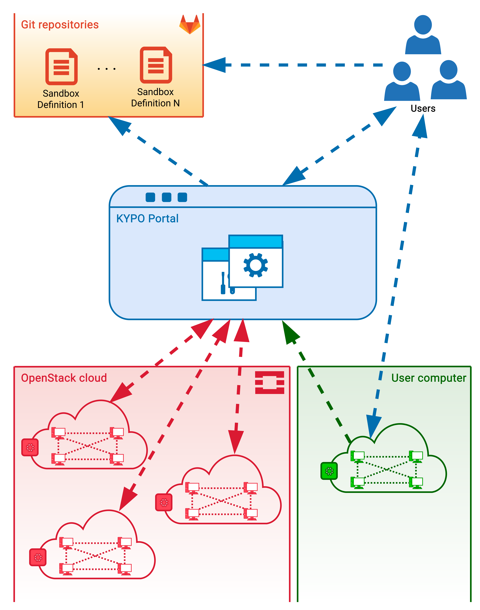
\includegraphics[width=0.7\linewidth]{kypo.png}
    \caption{Konzeptionelle Architektur von KYPO - Quelle: \cite{KYPOConceptualArchitecture}}
    \label{fig:kypo-conceptual-architecture}
\end{figure}

Abbildung~\ref{fig:kypo-conceptual-architecture} zeigt die Grundidee von KYPO in vereinfachter Form:
\emph{Sandbox-Definitionen} werden in Git-Repositories versioniert abgelegt. Das \emph{KYPO Portal}
dient als zentrale Komponente für die Verwaltung und nutzt diese Definitionen, um die
entsprechenden Ressourcen in einer \emph{OpenStack-Cloud} bereitzustellen. Nutzer greifen anschließend
von ihren Endgeräten auf die erzeugten Sandboxes zu.

Aus funktionaler Sicht übernimmt KYPO damit insbesondere (1) die Verwaltung von Sandbox-Definitionen
und deren Versionierung über Git, (2) die Orchestrierung und Bereitstellung der Umgebungen in OpenStack
sowie (3) den Zugang und die Nutzung der bereitgestellten Umgebungen durch Benutzer über das Portal.

\subsection{CyberRangeCZ}
\label{subsec:cyberrangecz}

CyberRangeCZ ist eine Open-Source-Plattform zur Erstellung und 

szenariobasierter Cyber-Range-Übungen mit dynamischer Bereitstellung von isolierten
Umgebungen (\emph{Sandboxes}). Die Plattform wird als Weiterentwicklung der KYPO Cyber
Range Platform (KYPO CRP) beschrieben und baut konzeptionell auf deren Ansatz auf,
während die technische Umsetzung stärker auf moderne, containerisierte Komponenten
und automatisierbare Bereitstellung ausgerichtet ist \cite{CyberRangeCZCyberRanges,CyberRangeCZGitHub}.

Aus architektonischer Sicht wird CyberRangeCZ als containerbasierte Microservices-Plattform
dargestellt. Zentrale Bausteine sind dabei insbesondere ein Sandbox Service zur
Lebenszyklusverwaltung der bereitgestellten Umgebungen sowie Trainingsdienste für
lineare und adaptive Trainingspfade (inklusive Unterstützung für Feedback- und
Auswertungsfunktionen) \cite{CyberRangeCZGitHub}.
Die Bereitstellung der Workloads erfolgt laut Projektbeschreibung auf einer
Kombination aus Kubernetes und Cloud-Backends, wobei u.\,a. OpenStack und AWS als
Zielumgebungen genannt werden \cite{CyberRangeCZGitHub}.

Ein wesentliches Merkmal der Plattform ist, dass die Bereitstellung und Konfiguration
stark automatisierungsorientiert beschrieben wird. In den Repositories finden sich dazu
u.\,a. Artefakte und Deploymentskripte, die auf gängigen IaC- und Cluster-Mechanismen
aufbauen (z.\,B. Helm-basierte Deployments), wodurch sich Installationen und Umgebungen strukturiert
wiederholbar aufsetzen lassen \cite{CyberRangeCZGitHub,CyberRangeCZDocs}.

Für den praktischen Betrieb stellt CyberRangeCZ ein webbasiertes Portal zur Verfügung,
über das Benutzer und Trainings verwaltet und Sandboxes gestartet werden können.
Szenarien bzw.\ Trainingsdefinitionen werden als wiederverwendbare Artefakte gepflegt,
wodurch sich Konfigurationen versionieren und iterativ anpassen lassen \cite{CyberRangeCZGitHub}.
Darüber hinaus wird die Plattform explizit als Grundlage genannt, um externe
Werkzeuge in Übungen einzubinden bzw.\ Übungen so zu gestalten, dass eine Integration
mit Drittanbietertools möglich ist \cite{CyberRangeCZCyberRanges}. Neben der technischen Dokumentation ist die Plattform auch über öffentliche
Entwicklungs- und Austauschkanäle nachvollziehbar: Quellcode, Issue-Tracking und
Diskussionen sind zentral über die Projektorganisation gebündelt.
\cite{CyberRangeCZGitHub}.

\subsection{Open Cyber Range (OCR)}
\label{subsec:ocr}

Open Cyber Range (OCR) ist ein Open-Source-Ansatz zur Erstellung und zum Betrieb
von Cyber-Range-Umgebungen, bei dem wiederverwendbare Komponenten und
Szenariodefinitionen so organisiert werden, dass Umgebungen strukturiert bereitgestellt
und durchgeführt werden können \cite{OCRDocs,OCRGitHub}.
OCR wird dabei als selbst betreibbare Plattform dokumentiert, die den Aufbau von
Übungs- bzw.\ Experimentierumgebungen aus definierten Bausteinen unterstützt \cite{OCRDocs}.

Die Projektdokumentation beschreibt OCR als modularen Ansatz, bei dem zentrale
Funktionen für die Bereitstellung und Durchführung von Umgebungen über klar getrennte
Komponenten abgebildet werden. Der Quellcode und die Projektartefakte sind in mehreren
Repositories organisiert; damit sind Implementierung, Konfigurationsmechanismen und
Weiterentwicklung transparent nachvollziehbar \cite{OCRGitHub}.
Für die praktische Nutzung stellt OCR eine eigenständige Dokumentation bereit, in der
Installation, grundlegende Konzepte sowie der Umgang mit Szenarien und Komponenten
beschrieben werden \cite{OCRDocs}.








\chapter{Technische Erkundung: Proof-of-Concept mit CyberRangeCZ}
\label{chap:technische-erkundung}

Ziel der technischen Erkundung war es, die grundsätzliche Machbarkeit einer selbst betriebenen
Cyber-Range-Plattform im Sinne der späteren Masterarbeit zu überprüfen. Im Fokus stand dabei
kein umfassender Produktivbetrieb, sondern ein \emph{Proof-of-Concept} (PoC), der zentrale
Abläufe demonstriert: Installation und Deployment der Plattform, Erstzugriff über die Weboberflächen,
Import einer Trainingsdefinition, Bereitstellung einer Sandbox sowie der Zugriff auf die bereitgestellten
Systeme.

Für den PoC wurde die CyberrangeCZLite-Variante verwendet, da sie einen schnellen Einstieg in die
Plattformmechanik ermöglicht und zugleich die wesentlichen Konzepte (Portal, Trainingsdefinitionen,
Pools, Sandboxes) abbildet \cite{CyberRangeCZDevopsLite}.

\section{Testumgebung}
\label{sec:poc-testumgebung}

Der PoC wurde auf einer dedizierten Maschine mit Ubuntu 24.04 LTS durchgeführt. Die verwendeten
Ressourcen (CPU, RAM und Storage) sind in Abbildung~\ref{fig:poc-hardware} dargestellt.


\begin{figure}[H]
    \centering
    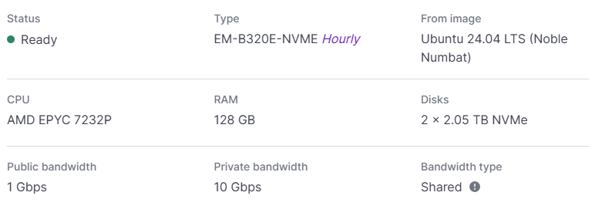
\includegraphics[width=0.85\linewidth]{poc_hardware.png}
    \caption{Testumgebung für den PoC (eigene Aufnahme)}
    \label{fig:poc-hardware}
\end{figure}

\section{Installation und Deployment der PoC-Umgebung}
\label{sec:poc-installation}

Die Installation folgt dem Ansatz, notwendige Virtualisierungs- und Container-Komponenten
lokal bereitzustellen und das eigentliche Deployment über das bereitgestellte PoC-Repository
automatisiert auszuführen. Dazu wurden zunächst Basiswerkzeuge sowie KVM/libvirt und Docker
installiert. KVM/libvirt stellt die Virtualisierungsbasis bereit (VM-Lifecycle und Netzwerk),
während Docker genutzt wird, um eine vorbereitete Umgebung auszuführen, in der eine vagrant
mit libvirt-Anbindung zur Provisionierung verwendet wird.

\begin{verbatim}
sudo apt install -y \
  git tmux curl \
  qemu-kvm libvirt-daemon-system libvirt-clients bridge-utils cpu-checker \
  docker.io
\end{verbatim}

Im nächsten Schritt wurden die relevanten Dienste aktiviert und der Benutzer für die Verwendung von
\texttt{libvirt}, KVM und Docker berechtigt. Damit wird erreicht, dass Virtualisierung und Containerbetrieb
ohne ständige Root-Kontexte nutzbar sind.

\begin{verbatim}
sudo systemctl enable --now libvirtd docker
sudo usermod -aG libvirt,kvm,docker $USER
newgrp docker
\end{verbatim}

Anschließend wurde das PoC-Repository geklont und die libvirt-URI gesetzt, sodass Vagrant eindeutig
die System-libvirt-Instanz adressiert. Zur langlebigen Durchführung lange Laufzeit, viele Ausgaben
wurde der Prozess in einer tmux-Session gestartet.

\begin{verbatim}
git clone https://github.com/cyberrangecz/devops-crczp-lite.git
cd devops-crczp-lite
export LIBVIRT_DEFAULT_URI=qemu:///system
tmux new -s crczp
\end{verbatim}

Das eigentliche Deployment erfolgt über einen Docker-Container, der Vagrant mit libvirt-Unterstützung
bereitstellt. Die relevanten Sockets und Verzeichnisse werden in den Container gemountet, damit Vagrant
(1) auf libvirt zugreifen kann, (2) seine Vagrant-States dauerhaft speichern kann und (3) im aktuellen
Arbeitsverzeichnis die Definitionsdateien findet. Der Parameter --network host stellt sicher, dass
Netzwerkoperationen und lokale Zugriffe (z.\,B. auf die Weboberfläche) ohne zusätzliche Container-NAT-
Komplexität funktionieren.

\begin{verbatim}
docker run -it --rm \
  -e LIBVIRT_DEFAULT_URI \
  -v /var/run/libvirt/:/var/run/libvirt/ \
  -v ~/.vagrant.d:/.vagrant.d \
  -v $(realpath "${PWD}"):${PWD} \
  -w "${PWD}" \
  --network host \
  vagrantlibvirt/vagrant-libvirt:latest \
  vagrant up
\end{verbatim}

Nach erfolgreichem Abschluss wurde eine URL für das Web-Portal sowie initiale Zugangsdaten ausgegeben.
Diese Ausgabe ist in Abbildung~\ref{fig:poc-deploy} dokumentiert. 


\begin{figure}[H]
    \centering
    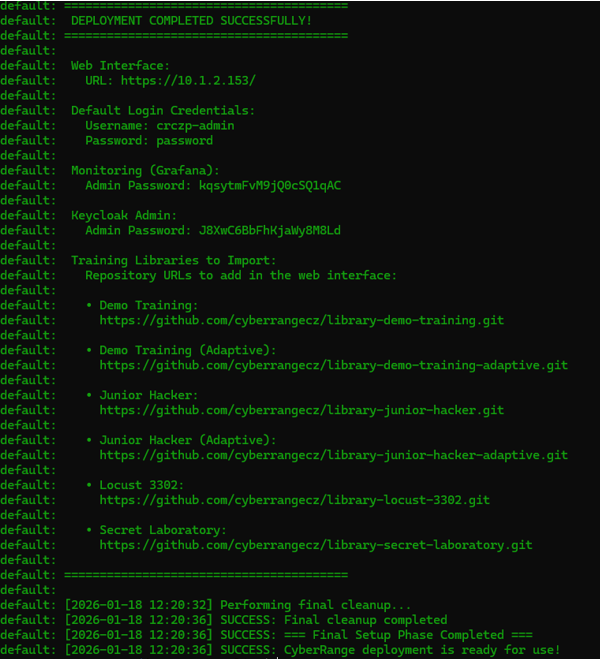
\includegraphics[width=0.92\linewidth]{poc_deploy_done.png}
    \caption{Erfolgreiches Deployment der PoC-Umgebung (eigene Aufnahme)}
    \label{fig:poc-deploy}
\end{figure}

\section{Erstzugriff über Keycloak und CyberRangeCZ-Portal}
\label{sec:poc-webzugriff}

CyberRangeCZ verwendet für Authentifizierung und Benutzer-/Client-Verwaltung typischerweise
Keycloak als Identity- und Access-Management-Komponente. Der erfolgreiche Zugriff auf die
Keycloak-Verwaltungskonsole bestätigt, dass die Authentifizierungs- und Basisdienste funktionsfähig
bereitgestellt wurden (Abbildung~\ref{fig:poc-keycloak}).


\begin{figure}[H]
    \centering
    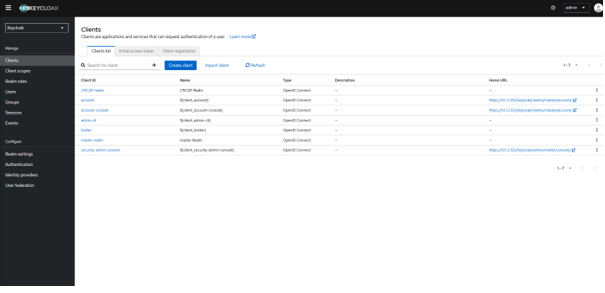
\includegraphics[width=0.95\linewidth]{poc_keycloak.png}
    \caption{Keycloak-Verwaltungskonsole der PoC-Installation(eigene Aufnahme)}
    \label{fig:poc-keycloak}
\end{figure}

Der zentrale Einstiegspunkt für Trainings- und Sandbox-Management ist das CyberRangeCZ Platform Portal.
Abbildung~\ref{fig:poc-portal} zeigt die Startseite und zeigt die wichtigsten Funktionen,
u.\,a.\ Trainingsdefinitionen, Trainingsinstanzen, Sandboxes, Pools sowie Benutzer- und Gruppenverwaltung.


\begin{figure}[H]
    \centering
    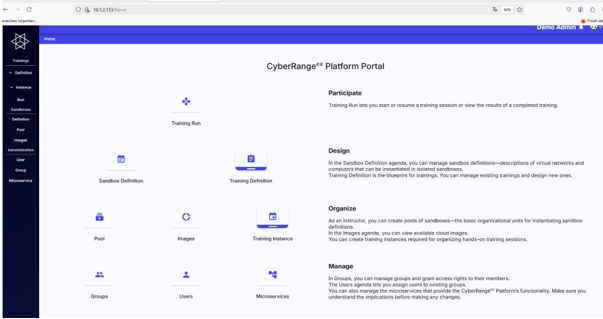
\includegraphics[width=0.95\linewidth]{poc_portal_home.png}
    \caption{CyberRangeCZ Platform Portal (Startseite) nach erfolgreichem Login(eigene Aufnahme)}
    \label{fig:poc-portal}
\end{figure}

\section{Import einer Trainingsdefinition und Provisionierung einer Sandbox}
\label{sec:poc-training-import}

Um die Kernfunktionalität der Plattform zu validieren, wurde eine Beispiel-Trainingsbibliothek
(\emph{library-demo-training}) aus einem Git-Repository in das Portal eingebunden \cite{CyberRangeCZLibraryDemoTraining}. Nach dem Import wurde ein Pool bzw.\ eine Trainingsinstanz erstellt und die Sandbox-Provisionierung
ausgelöst. Die resultierende Netzwerktopologie der bereitgestellten Umgebung ist in
Abbildung~\ref{fig:poc-topology} dargestellt.


\begin{figure}[H]
    \centering
    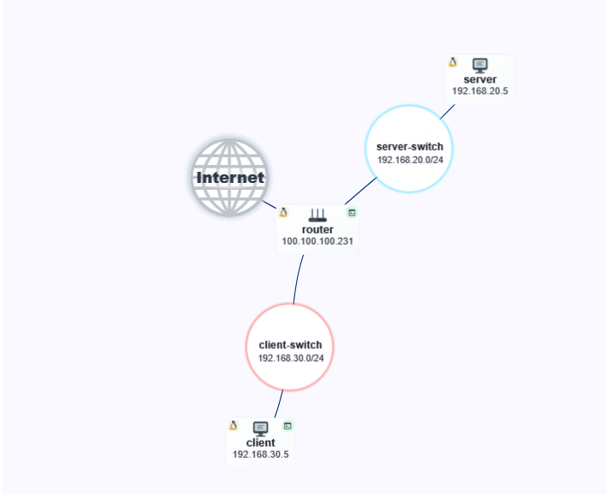
\includegraphics[width=0.80\linewidth]{poc_topology.png}
    \caption{Netzwerktopologie einer bereitgestellten Demo-Sandbox (eigene Aufnahme)}
    \label{fig:poc-topology}
\end{figure}

\section{Zugriff auf die Sandbox und funktionaler Verbindungstest}
\label{sec:poc-zugriff}

Für den Zugriff auf die bereitgestellten Systeme stellt CyberRangeCZ im PoC automatisch erzeugte
SSH-Artefakte zur Verfügung. Dazu gehören typischerweise eine Benutzer-Konfiguration sowie ein
passender privater und öffentlicher Schlüssel. Abbildung~\ref{fig:poc-ssh-files} zeigt
die entsprechenden Dateien, die nach der Sandbox-Provisionierung bereitgestellt wurden.

Neben SSH sind in Cyber-Range-Umgebungen grundsätzlich auch weitere Zugriffsmöglichkeiten relevant,
insbesondere wenn Trainings- oder Forschungsszenarien eine grafische Interaktion erfordern. Je nach
Szenariodefinition kann der Zugriff daher auch über browserbasierte Oberflächen bzw.\ GUI-Zugriffe
(z.\,B.\ über eine Web-Konsole oder Remote-Desktop-Mechanismen wie RDP/VNC/noVNC) erfolgen.
Welche Zugriffspfade tatsächlich verfügbar sind, hängt dabei von der jeweiligen Trainingsdefinition
und der bereitgestellten Infrastruktur ab.


\begin{figure}[H]
    \centering
    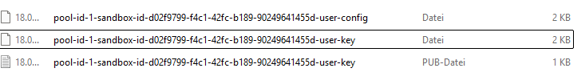
\includegraphics[width=0.90\linewidth]{poc_ssh_files.png}
    \caption{SSH-Daten für den Sandbox-Zugriff (eigene Aufnahme)}
    \label{fig:poc-ssh-files}
\end{figure}

Zur Verifikation, dass der Zugriff auf die Sandbox tatsächlich funktioniert und Netzwerkkommunikation
möglich ist, wurde aus der bereitgestellten Client-Umgebung ein einfacher Scan gegen das Server-System
durchgeführt. Abbildung~\ref{fig:poc-nmap} zeigt exemplarisch, dass das Zielsystem erreichbar ist und
SSH (Port 22) offen ist. Damit ist die grundlegende Nutzbarkeit der bereitgestellten Umgebung für
weitere Schritte nachgewiesen.


\begin{figure}[H]
    \centering
    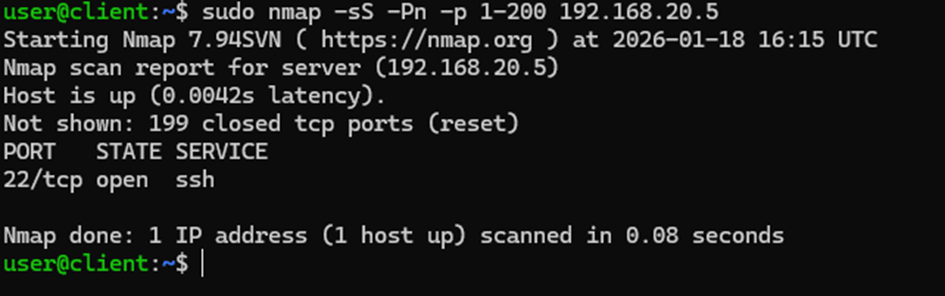
\includegraphics[width=0.92\linewidth]{poc_nmap.png}
    \caption{Einfacher Funktionstest innerhalb der Sandbox (eigene Aufnahme)}
    \label{fig:poc-nmap}
\end{figure}

\section{Erkenntnisse aus dem PoC}
\label{sec:poc-erkenntnisse}

Der PoC bestätigt, dass CyberRangeCZ (in der Lite-Variante) in einer lokalen Umgebung
installiert und betrieben werden kann und dabei zentrale Plattformmechanismen bereits sichtbar werden:
versionierbare Trainingsdefinitionen, Portal-gestützte Verwaltung sowie automatisierte Provisionierung
isolierter Umgebungen. Für das Vorprojekt ist insbesondere relevant, dass sich eine Trainingsdefinition
aus einem Git-Repository importieren und anschließend reproduzierbar als Sandbox instanziieren lässt.

Für die Masterarbeit ergibt sich daraus als nächster Schritt, die technische Erkundung in Richtung
Tool-Integration zu vertiefen, d.\,h.\ konkrete Mess- und Beobachtungspunkte (Logs, Metriken,
Netzwerkdaten) in einem Use-Case gezielt zu platzieren und den Aufwand für Integration und Vergleich
mehrerer Sicherheits- bzw.\ Monitoring-Werkzeuge realistisch abzuschätzen.

\chapter{Technische Erkundung: Proof-of-Concept mit Open Cyber Range (OCR)}
\label{chap:poc-ocr}

Ziel dieser technischen Erkundung war es, neben CyberRangeCZ eine zweite Open-Source-Cyber-Range-Plattform praktisch zu evaluieren.
Im Vordergrund stand dabei kein Produktivbetrieb, sondern ein nachvollziehbarer Proof-of-Concept (PoC), der zeigt, ob sich OCR auf
einem Host deployen lässt und wie die Plattformarchitektur in der Praxis handhabbar ist.

Im Unterschied zu vielen ``All-in-one''-Trainingsplattformen ist OCR nicht als monolithisches Webprodukt konzipiert, sondern als
Baukastensystem aus mehreren Diensten, die gemeinsam den Lebenszyklus einer Übung abdecken: (1) Verwaltung und Distribution von
Übungsartefakten, (2) Orchestrierung und Zustandsverwaltung von Deployments, (3) Anbindung an eine konkrete Infrastruktur
(Virtualisierung/Cloud) sowie (4) Identity- und Access-Management. Diese modulare Architektur ist für Forschung prinzipiell attraktiv,
erhöht im Self-Hosted-Betrieb jedoch den Integrationsaufwand erheblich, da mehrere Komponenten konsistent konfiguriert und miteinander verbunden
werden müssen \cite{OCRDeputyRepo,OCRCZRangerDoc}.

Für den PoC wurden die Kernkomponenten Deputy und die Ranger-Komponente betrachtet. Deputy fungiert als digitale Bibliothek
für Szenarioinhalte: Artefakte (z.\,B.\ Packages, Templates oder vorbereitete Übungskomponenten) werden dort versioniert
abgelegt und können von anderen OCR-Komponenten abgerufen werden.\cite{OCRDeputyRepo,OCRCZFirstDeputyPackage}.

Die Ranger-Komponente bildet die Control Plane für die Ausführung: Sie verwaltet den Zustand einer Übung und koordiniert das
Ausrollen in eine Zielumgebung. Entscheidend ist dabei, dass Ranger die Infrastruktur nicht selbst erzeugt, sondern die Provisionierung
an umgebungsspezifische Handler/Deployer delegiert. OCR bildet damit einen Datenfluss ab: Für OpenStack existiert ein eigener Handler als separates Projekt \cite{OCROpenstackHandler}

\section{Testumgebung}
\label{sec:poc-ocr-testumgebung}

Der PoC wurde auf einer dedizierten Maschine mit Ubuntu 24.04 LTS durchgeführt. Die verwendeten Ressourcen (CPU, RAM und Storage) sind in Abbildung~\ref{fig:poc-ocr-hardware} dargestellt.

\begin{figure}[H]
    \centering
    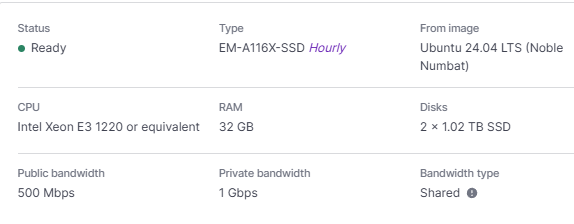
\includegraphics[width=0.85\linewidth]{poc_ocr_hardware.png}
    \caption{Testumgebung für den OCR-PoC (eigene Aufnahme)}
    \label{fig:poc-ocr-hardware}
\end{figure}

\section{Installation und Deployment der PoC-Umgebung}
\label{sec:poc-ocr-installation}

Die Installation orientierte sich grundsätzlich an der offiziellen Cyber-Range-Dokumentation für die OCR-Komponenten (Deputy und Ranger) \cite{OCRCZRangerDoc,OCRCZFirstDeputyPackage}. In der praktischen Umsetzung kamen aber viele Probleme auf die nicht in der Dokumentation standen: Der Ranger-Service beispielsweiße, prüft beim Start die Konfiguration strikt auf Vollständigkeit und korrekte Datentypen. Fehlende Pflichtfelder (z.\,B.\ für Deployer-/Deployment-Strukturen, ...) führten daher zu wiederholten Startabbrüchen und Neustartschleifen. 

\subsection{Deployment von Deputy}
\label{subsec:poc-ocr-deputy}

Deputy wurde als erster Baustein gestartet, da Ranger für den späteren Betrieb typischerweise Artefakte über Deputy bezieht.
Der Start erfolgte über Docker Compose. Abbildung~\ref{fig:poc-ocr-deputy-up} dokumentiert den erfolgreichen Image-Pull und die laufendenContainer.

\begin{verbatim}
cd /opt/ocr/deputy
docker compose up -d
docker ps
\end{verbatim}

\begin{figure}[H]
    \centering
    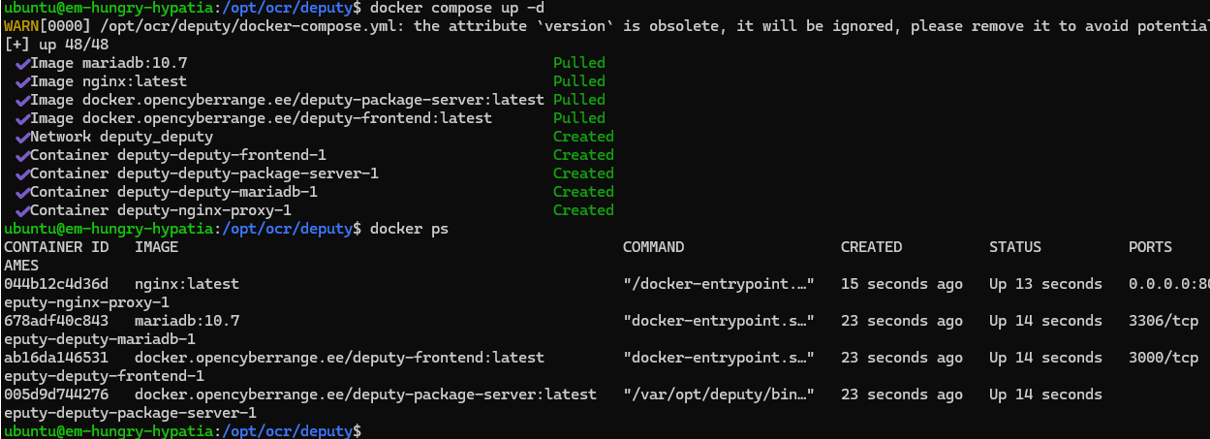
\includegraphics[width=1\linewidth]{poc_ocr_deputy_up.png}
    \caption{Deputy: erfolgreicher Start der Services (eigene Aufnahme)}
    \label{fig:poc-ocr-deputy-up}
\end{figure}

\subsection{Deployment der Ranger-Komponente}
\label{subsec:poc-ocr-ranger}

Im nächsten Schritt wurde die Ranger-Komponente deployt. In der Praxis erwies sich dieser Teil als deutlich aufwändiger als erwartet,
da Ranger bereits im Minimalbetrieb strikte Anforderungen an die Konfiguration stellt. Ranger validiert beim Start eine Reihe
verpflichtender Felder und Datentypen. Fehlen diese Angaben oder passen sie nicht exakt, beendet sich der Dienst sofort mit
Fehlermeldungen. 

Der Start und der Containerstatus sind in Abbildung~\ref{fig:poc-ocr-ranger-up} dokumentiert. Abbildung~\ref{fig:poc-ocr-ranger-logs}
zeigt den erfolgreichen Start über Logmeldungen des Webservers (Actix startet Worker).

\begin{figure}[H]
    \centering
    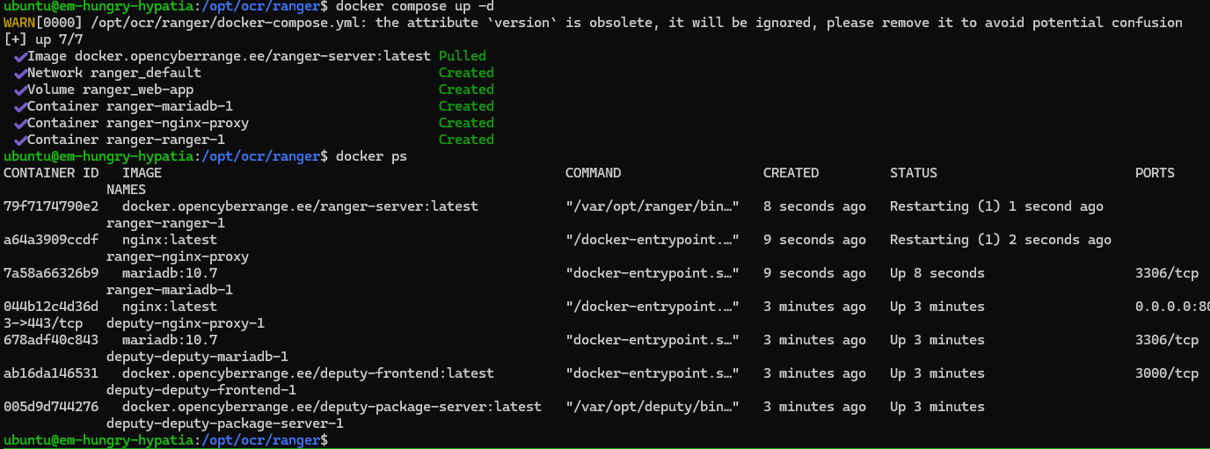
\includegraphics[width=1\linewidth]{poc_ocr_ranger_up.png}
    \caption{Ranger-Komponente(eigene Aufnahme)}
    \label{fig:poc-ocr-ranger-up}
\end{figure}

\begin{figure}[H]
    \centering
    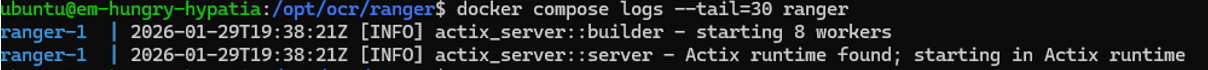
\includegraphics[width=1\linewidth]{poc_ocr_ranger_logs.png}
    \caption{Ranger-Komponente: erfolgreicher Start (eigene Aufnahme)}
    \label{fig:poc-ocr-ranger-logs}
\end{figure}


Im Rahmen des Vorprojekts konnte der Proof-of-Concept für die Open Cyber Range (OCR) in der verfügbaren Zeit nicht bis zu einem lauffähigen Trainings-/Deployment-Start abgeschlossen werden. Obwohl zentrale Komponenten (Deputy und Ranger) grundsätzlich gestartet werden konnten, erwies sich die praktische Integration der modularen OCR-Architektur deutlich komplexer als erwartet, da mehrere Dienste (u.,a. Identity- und Access-Management) konfiguriert und miteinander abgestimmt werden müssen. Zusätzlich setzt die eigentliche Bereitstellung von Übungsumgebungen eine angebundene Virtualisierungs- bzw. Cloud-Infrastruktur voraus (z.,B. eine eigene OpenStack-Umgebung oder alternativ VMware/ESXi über passende Handler/Deployer). Der PoC bleibt daher auf den erfolgreichen Aufbau der Basisservices und die technische Erkundung der Architektur beschränkt.
\chapter{Kriterienkatalog zur Plattformbewertung}

\section{Kriterienkatalog für die Plattformbewertung}
\label{sec:kriterienkatalog}

Um im Vorprojekt eine nachvollziehbare und später begründbare Vorauswahl treffen zu können,
wird ein Kriterienkatalog definiert, anhand dessen die betrachteten Open-Source-Cyber-Ranges
strukturiert beschrieben und bewertet werden. Der Katalog ist so gewählt, dass er die späteren
Ziele der Masterarbeit abbildet, ohne dabei bereits eine bestimmte Plattform vorauszusetzen.
Die Kriterien dienen im weiteren Verlauf als Grundlage für die vergleichende Analyse und für
eine begründete Empfehlung.

\textbf{K1 -- Reproduzierbarkeit und Wiederholbarkeit:}
Kann die Plattform identische Umgebungen und Szenarien in gleicher Konfiguration wiederholt bereitstellen
(z.\,B.\ durch versionierbare Definitionen und deterministische Provisionierung)?

\textbf{K2 -- Automatisierung und Lifecycle-Steuerung:}
Unterstützt die Plattform den Lifecycle von Umgebungen (Provisionierung, Start/Stop, Reset, Cleanup)
weitgehend automatisiert und mit geringem manuellem Betriebsaufwand?

\textbf{K3 -- Integrationsfähigkeit externer Werkzeuge:}
Erlaubt die Plattform die Einbindung zusätzlicher Tools innerhalb der Sandbox oder am Rand der Umgebung
(z.\,B.\ Sensoren, Agents, SIEM/Logging, Monitoring), sodass Vergleiche unter gleichen Bedingungen möglich sind?

\textbf{K4 -- Beobachtbarkeit und Datenzugang:}
Stellt die Plattform Mechanismen bereit, um Mess- und Auswertungsdaten systematisch zu erfassen und zugänglich zu machen
(z.\,B.\ Logs, Metriken, Events, Netzwerkdaten) und diese für Analysen zu exportieren bzw.\ weiterzuverarbeiten?

\textbf{K5 -- Zugriffsmöglichkeiten und Nutzerinteraktion:}
Bietet die Plattform praktikable Zugriffsmöglichkeiten auf die bereitgestellten Systeme (z.\,B.\ SSH sowie optional GUI-/Web-Konsole/RDP/VNC)
und unterstützt sie eine nutzerfreundliche Interaktion während der Durchführung?

\textbf{K6 -- Benutzer-, Rollen- und Rechteverwaltung:}
Unterstützt die Plattform Mehrbenutzerbetrieb mit Rollen- und Gruppenkonzepten, nachvollziehbarer Zugriffskontrolle
und klaren Mechanismen für Authentisierung/Autorisierung?

\textbf{K7 -- Wartbarkeit, Dokumentation und Community:}
Ist die Plattform realistisch betreib- und wartbar (z.\,B.\ nachvollziehbarer Installations-/Update-Prozess),
gut dokumentiert und durch aktive Weiterentwicklung bzw.\ Austausch-/Support-Kanäle unterstützt?\newline
\newline



\chapter{Vergleichsmatrix}

\begin{table}[H]
\centering
\renewcommand{\arraystretch}{1.2}
\begin{tabular}{p{5.2cm}ccc}
\hline
\textbf{Kriterium} & \textbf{CyberRangeCZ} & \textbf{OCR} & \textbf{KYPO} \\
\hline
\textbf{K1 Reproduzierbarkeit \& Wiederholbarkeit}      & \cmark & \cmark & \cmark \\
\textbf{K2 Automatisierung \& Lifecycle-Steuerung}       & \cmark & $\sim$ & \cmark \\
\textbf{K3 Integrationsfähigkeit externer Werkzeuge}     & $\sim$ & ?      & ?      \\
\textbf{K4 Beobachtbarkeit \& Datenzugang}                    & \cmark & ? & \cmark \\
\textbf{K5 Zugriffsmöglichkeiten \& Nutzerinteraktion}   & \cmark & ?      & \cmark \\
\textbf{K6 Benutzer-, Rollen- \& Rechteverwaltung}       & \cmark & \cmark & \cmark \\
\textbf{K7 Wartbarkeit, Dokumentation \& Community}      & \cmark & $\sim$ & \xmark \\
\hline
\end{tabular}
\caption{Vergleichsmatrix der Plattformen anhand der Kriterien K1--K7 (\cmark\ erfüllt, $\sim$ teilweise erfüllt, \xmark\ nicht erfüllt, ? offen).}
\label{tab:plattformvergleich-matrix}
\end{table}
Die Vergleichsmatrix in Tabelle~\ref{tab:plattformvergleich-matrix} zeigt, dass CyberRangeCZ im Vorprojekt in mehreren für die spätere Masterarbeit zentralen Kriterien bereits nachweisbar stark abschneidet. Insbesondere die praktische Erprobung im PoC belegt einen hohen Grad an Automatisierung und Lifecycle-Steuerung (K2) sowie praktikable Zugriffsmöglichkeiten und Nutzerinteraktion (K5). Auch Aspekte des Mehrbenutzerbetriebs und der Zugriffskontrolle (K6) sind durch die vorhandenen Plattformkomponenten und das Portal-Konzept klar adressiert. Zusammen mit der umfangreichen Dokumentation und aktiven Weiterentwicklung (K7) reduziert dies das Umsetzungsrisiko für die Masterarbeit.

KYPO erfüllt konzeptionell ebenfalls wesentliche Anforderungen, insbesondere hinsichtlich reproduzierbarer Umgebungen und automatisierter Bereitstellung (K1, K2), basiert jedoch auf einer älteren technischen Architektur und wird im Projektkontext zunehmend durch CyberRangeCZ abgelöst. Dadurch entsteht im Vergleich ein Nachhaltigkeitsrisiko (K7), das für eine längerfristige Forschungsumgebung in einer Masterarbeit relevant ist. OCR verfolgt einen modularen, standardorientierten Ansatz , jedoch konnten zentrale Punkte im Vorprojekt nicht in gleicher Tiefe praktisch verifiziert werden. Entsprechend werden einzelne Kriterien als \emph{teilweise erfüllt} bzw.\ \emph{offen} bewertet. Dies betrifft vor allem die konkrete technische Bereitstellung einer vollständigen Übungskette im PoC sowie die daraus ableitbare Beurteilung einzelner Betriebs- und Zugriffsaspekte. Zusätzlich wirkt die verfügbare Dokumentation im Vergleich weniger umfassend und die Community-Aktivität bzw.\ der Austausch über Support-Kanäle ist weniger ausgeprägt, was die Fehlersuche und den Wissenstransfer im Implementierungsprozess potenziell erschwert.

\chapter{Vorläufige Auswahl der Plattform}
\label{chap:auswahl}

Ziel des Vorprojekts ist keine endgültige Festlegung, sondern eine begründete Vorauswahl, die die spätere Umsetzung der Masterarbeit ermöglicht. Die Entscheidung stützt sich auf den Kriterienkatalog (Kapitel~\ref{sec:kriterienkatalog}) und die vergleichende Einordnung in Tabelle~\ref{tab:plattformvergleich-matrix}. 

\section{Gewichtung der Kriterien}
Für das Forschungsvorhaben stehen Reproduzierbarkeit und Wiederholbarkeit (K1), Automatisierung und Lifecycle-Steuerung (K2), Integrationsfähigkeit externer Werkzeuge (K3) sowie Beobachtbarkeit und Datenzugang (K4) im Vordergrund, da sie die Vergleichbarkeit von Experimenten und die spätere Evaluation von Cyber-Resilienz-Use-Cases direkt beeinflussen. Benutzer-, Rollen- und Rechteverwaltung (K6) sowie Wartbarkeit, Dokumentation und Community (K7) sind ebenfalls wesentlich, weil sie die langfristige Nutzbarkeit und den stabilen Betrieb einer Forschungsumgebung beeinflussen. Zugriffsmöglichkeiten (K5) werden unterstützend berücksichtigt, da sie die praktische Durchführbarkeit von Übungen und Experimenten maßgeblich erleichtern.

\section{Begründete Vorauswahl}
Aus Tabelle~\ref{tab:plattformvergleich-matrix} ergibt sich CyberRangeCZ als die im Vorprojekt am robustesten begründbare Option. Im Unterschied zu den Alternativen konnten zentrale Kriterien nicht nur anhand von Dokumentation, sondern zusätzlich durch den erfolgreich umgesetzten PoC praktisch untermauert werden. Damit liegen belastbare Hinweise vor, dass die Plattform den automatisierten Aufbau und Betrieb von Umgebungen (K2) sowie einen praktikablen Zugriff und die Durchführung von Trainingsinstanzen (K5) unterstützt. Darüber hinaus sprechen die aktuelle Weiterentwicklung, die verfügbare Dokumentation und Support-/Community-Strukturen (K7) sowie die vorhandenen Mechanismen für Mehrbenutzerbetrieb und Zugriffskontrolle (K6) für ein geringeres Implementierungs- und Betriebsrisiko im Verlauf der Masterarbeit.

KYPO wird als fachlich relevanter Vorgängeransatz eingeordnet, weist jedoch im Vergleich ein erhöhtes Nachhaltigkeitsrisiko auf, da es als Vorgängerprojekt gilt und der Schwerpunkt der Weiterentwicklung auf CyberRangeCZ liegt. OCR stellt zwar einen interessanten modularen Ansatz dar, konnte im Vorprojekt jedoch nicht in allen für die Auswahl entscheidenden Punkten praktisch verifiziert werden. Entsprechend wird OCR für die Masterarbeit vorerst nicht als primäre Zielplattform gewählt, kann aber als Referenz für sowie für eine mögliche spätere Erweiterung oder Gegenüberstellung herangezogen werden.

Auf Basis der Kriteriengewichtung und der im Vorprojekt gewonnenen Erkenntnis wird daher CyberRangeCZ als vorläufige Zielplattform für die Masterarbeit ausgewählt.

\chapter{Ausblick auf die Masterarbeit}

In der Masterarbeit ist eine Evaluation der Cyber Range als Forschungsumgebung anhand
reproduzierbarer Cyber-Resilienz-Use-Cases vorgesehen. Der Kern der Evaluation ist ein
vergleichbarer Aufbau: Für jeden Use Case wird ein klar definierter Ausgangszustand
festgelegt und über wiederholte Läufe identisch
bereitgestellt. Auf dieser Basis sollen unterschiedliche Werkzeuge oder Werkzeugkonfigurationen
unter denselben Rahmenbedinungen gegenübergestellt werden. Dabei wird pro Vergleichslauf
jeweils nur die Werkzeugkomponente variiert, während Szenarioablauf, Datenquellen und
Messpunkte konstant bleiben.

Um die Vergleichbarkeit sicherzustellen, wird pro Use Case vorab festgelegt, welche
Beobachtungen als erwartete Ergebnisse gelten und wie diese überprüft werden.
Praktisch bedeutet das, dass für jeden Szenariolauf eine definierte Menge an
sicherheitsrelevanten Ereignissen bzw.\ Artefakten erzeugt wird (z.\,B.\ Port-Scan, Login-Versuche,
unerwartete Prozessstarts oder verdächtige Netzwerkverbindungen) und anschließend geprüft wird,
ob und in welcher Form die eingesetzten Werkzeuge diese Aktivitäten erkennen und sichtbar machen.
Die Auswertung kann dabei u.\,a. umfassen, (1) welche Events/Indikatoren vom Werkzeug tatsächlich
gemeldet wurden, (2) wie schnell eine Meldung nach dem Ereignis erfolgt, (3) wie viele irrelevante
Meldungen (False Positives) entstehen und (4) ob die bereitgestellten Kontextinformationen
für eine Interpretation und Nachvollziehbarkeit ausreichen (z.\,B.\ betroffener Host, Benutzer,
Zeitpunkt, technische Details). Durch wiederholte Läufe desselben Use Cases lässt sich zudem prüfen,
ob die Ergebnisse stabil reproduzierbar sind oder ob es zu signifikanten Abweichungen kommt.


Der Forschungsbeitrag entsteht dadurch, dass eine wiederholbare Experimentierumgebung geschaffen wird,
in der definierte Ereignisse reproduzierbar erzeugt werden können. Dadurch wird es möglich, Werkzeuge
nicht anhand einzelner Beobachtungen, sondern anhand wiederholter, vergleichbarer Läufe zu bewerten
(z.\,B.\ welche Aktivitäten erkannt werden, wie konsistent die Ergebnisse sind und welche Unterschiede
zwischen Werkzeugen auftreten).



%%%-----------------------------------------------------------------------------
\appendix                                                               % Anhang 
%%%-----------------------------------------------------------------------------

%%%\include{back/anhang_a} % Technische Ergänzungen
%%%\include{back/anhang_b} % Inhalt der CD-ROM/DVD
%%%\include{back/anhang_c} % Chronologische Liste der Änderungen
%%%\include{back/anhang_d} % Quelltext dieses Dokuments

%%%-----------------------------------------------------------------------------
\backmatter                          % Schlussteil (Quellenverzeichnis und dgl.)
%%%-----------------------------------------------------------------------------

\MakeBibliography % Quellenverzeichnis



%%%-----------------------------------------------------------------------------
\end{document}
%%%-----------------------------------------------------------------------------
